\label{ch:background}

A theoretical background is now presented, we first look at the methods of space transformation from bigger to lower dimensionality, and after a brief presentation of clustering methods that are used in one of the example of this project. 

\section{Space transformation}
\label{seq:space-transformation}

As previously mentioned, many proposed visualizations for spatio-temporal data uses an axis to represent the spatial distribution of data,
%
with the use of space transformation methods to represent the information contained in 2 dimensions in a 1D axis.
%
The transformation of space is a very common task in many domains with different properties depending on the objectives of the representation.

%
In this section will be presented a general overview of space transformation methods, 
%
separating in methods for dimensionality reduction of high-dimensional data and methods of spatial indexing that are heavily used in computer science.
%
A brief example of the different projection methods is presented in Fig.~\ref{fig:projection-example} on a dataset with two variables.

\begin{figure}
    \centering
    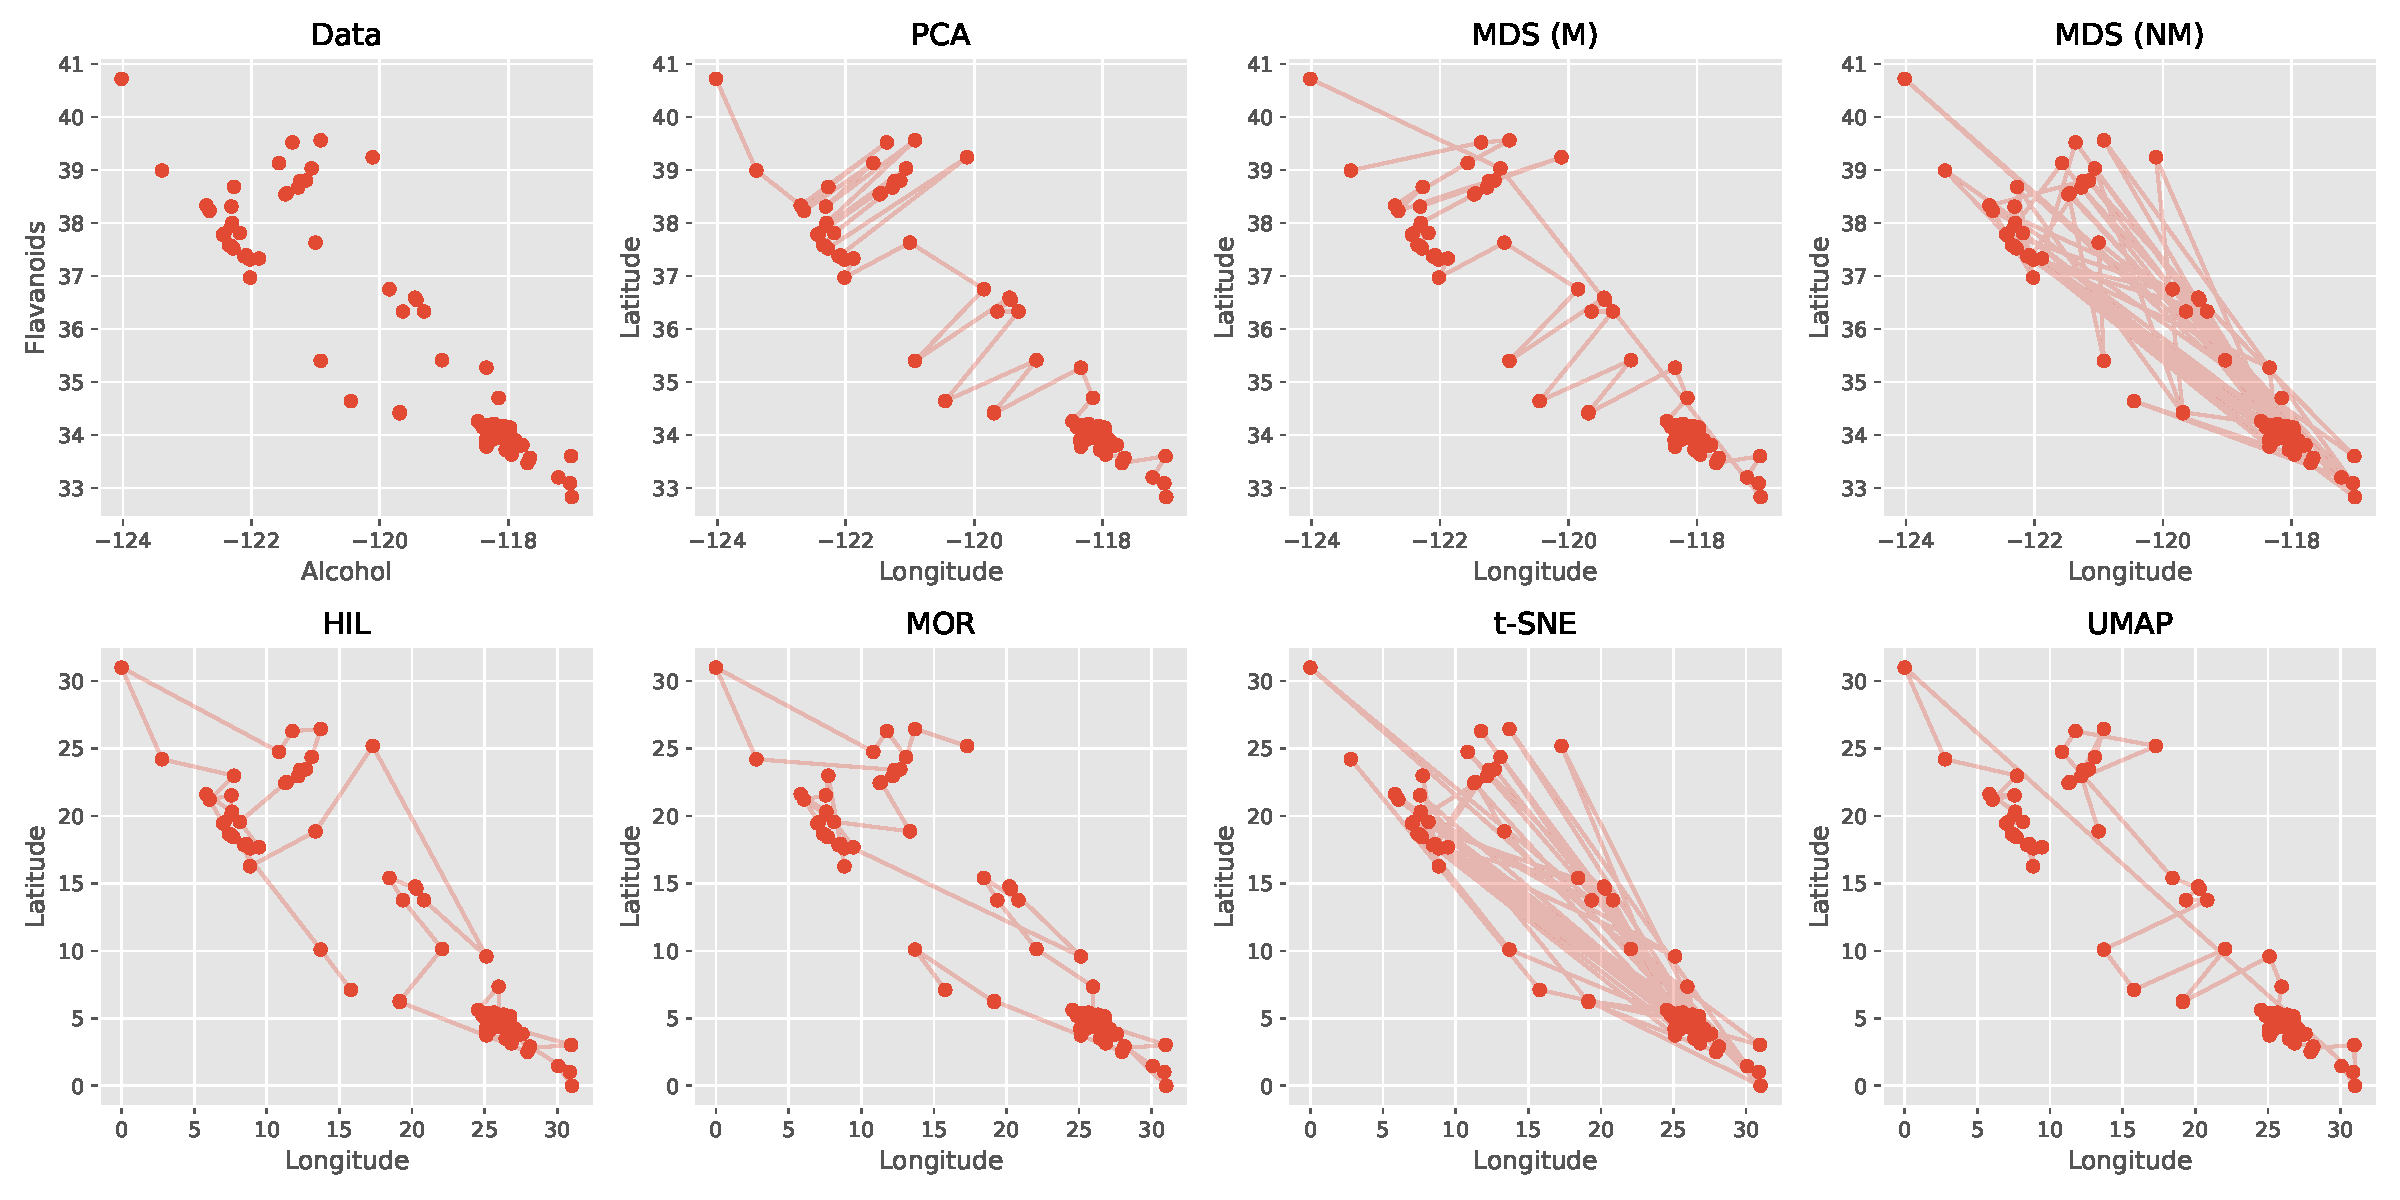
\includegraphics[width = \textwidth]{src/imgs/projection-example.pdf}
    \caption{Source: elaborated by author. Considered projection methods in an example dataset. The ordering of points is represented by the line connecting them, each point is connected to its predecessor and successor.}
    \label{fig:projection-example}
\end{figure}

\subsection{Dimensionality reduction}
%

With the recent advancements in technologies and means of communication, the availability, of high-dimensional data increased exponentially. 
%
Despite it great value of information, machine learning methods and algorithms can suffer from dimensionality problems.
%
Methods to represent the valuable information in lower dimensions have been developed and are vastly used.
%

Based on the overview presented by~\cite{ayesha2020dimensionality}, dimensionality reduction techniques are methods that transform high-dimensional data $Y = [y_1, \dots, y_m] \in \mathbb{R}^{m \times p}$ with dimension $p$ and $m$ samples to a new data in low dimensionality $Z = [z_1, \dots, z_m] \in \mathbb{R}^{k \times m}$ keeping the same $m$ samples but in a lower dimension, generally $k << p$. 
%

In this subsection will be presented the methods PCA, MDS, UMAP, and t-SNE.

\subsubsection{Principal Components Analysis}
%
PCA was first introduced by Pearson in 1901 and is one of the most studied methods of dimensionality reduction, and with many adaptations for different applications~\cite{ayesha2020dimensionality}.
%
The idea is that with p-dimensional data, there are dimensions that are of less interest when identifying different observations, so it is possible to reduce this dimensionality by maintaining only the dimensions with the greatest variance.
%
However, PCA is not a method for the selection of the features, what it does is to create new dimensions from a linear combination of the original $p$ dimensions, each of these created dimensions is called a \textit{principal component}.
%

With the same notation $Y\in \mathbb{R}^{m\times p}$, and $y_i \in \mathbb{R}^m, \forall i \in \{ 1, \dots, p\}$ the columns of $Y$, the first principal component is defined as~\cite{james2013introduction}:

\begin{equation*}
\begin{split}
    z_1 = \begin{cases}
    \argmax Var(z) \\
    z = \theta_{11}y_1 + \theta_{21}y_2 + \dots + \theta_{p1}y_p \\
    \sum_{i=1}^p\theta_{i1}^2 = 1
    \end{cases}
\end{split}
\end{equation*}

With $\theta_{1} = (\theta_{11}, \dots, \theta_{p1}) \in \mathbb{R}^p$ called \textit{loading}.
%
We can define the second principal component $z_2$ in a similar manner, a linear combination of $y_i$ that maximizes the variance, with normalized loading and with the additional constraint that $z_1$ and $z_2$ must be uncorrelated. 
%
Following $m = \min{(n -1 , p)}$ principal components can be defined in the same manner.
%

%
To apply PCA for space transformation, we generate a low dimensional $k$ representation of $Y$ in dimension $p$ by computing the first $k$ principal components and building a matrix with the components as columns $Z = [z_1, \dots, z_k]$, $z \in \mathbb{R}^{m\times k}$.
%
There are different manners to compute the loadings $\theta_i$ and following components, the most common being by using the eigenvectors from the covariance matrix of $Y$. 

\subsubsection{Multidimensional scaling}
%
MDS is a method similar to PCA, but the main difference is that instead of working with points in $\mathbb{R}^p$, 
%
MDS uses dissimilarity measures between pairs of points and tries to recreate a representation in a space of any dimension, generally low dimension, with the distances between points equal to the original dissimilarity measure.
%
The origin of this dissimilarity measure is not important for the method and can be any distance metric such as euclidean distance, Manhattan distance, or any other, per example, to obtain a 2D representation of the distance between cities of a country, it can be used the time necessary to travel by train between cities as a dissimilarity measure.
%
This presentation is based on the work from \cite{cox2008multidimensional}.
%

There are different versions of MDS, the most common are metric (or classical) and non-metric. 
%
Let $d_{i, j}$ be the dissimilarity measure between objects $i$ and $j$.
%
In the metric version, $d_{i, j}$ is interpreted as a distance value, although,
%
in the non-metric version, it is considered that $d_{i, j}$ does not fully represent a distance, and only the rank order of the value is used, i.e., the point farther from $i$ in the original space will be the farther in the calculated representation of $i$.
%

For a set of $m$ objects, with values $d_{i, j}$ defined above, a projection using MDS is a set of $m$ points in $\mathbb{R}^{p}$, usually with $p \in \{2, 3\}$, such that the euclidean distance between points $\hat d_{i, j}$ is close to $d_{i, j}$.
%
A metric to evaluate the goodness-of-fit is the stress measure defined as:

\begin{equation}
    S = \sqrt{\dfrac{\sum_{i = 1}^m \sum_{j = i + 1} ^m (d_{i, j} - \hat d_{i, j})^2}{\sum_{i = 1}^m \sum_{j = i + 1}^m  d_{i, j}}}
\end{equation}
\label{eq:stress-measure}

We have that $S \in [0, 1]$, and $S = 0$ means perfect representation and $S$ nears to $1$ means poor fitness.


%
To calculate the points, metric MDS apply a transformation in the matrix $D$ of dissimilarities and after uses the decomposition in eigenvalues and eigenvectors, similar to PCA. 
%
The non-metric version applies optimization algorithms in the stress metric.

\subsubsection{t-Distributed Stochastic Neighbor Embedding}
%
t-SNE~\cite{van2008visualizing} is one of the most used methods for visualizing high-dimensional data 
%
and compared with the other two mentioned methods,
%
it is a more advanced technique that creates probabilities of connections between points in the high-space and 
%
represents it in a low-space using the t-Student distribution.
%
We now present a general overview based on the great explanation in~\cite{stelling2019entendendo}.
%

Initially, with values $Y$ in high-space, the distance between points is computed and transformed to a probability using the Gaussian distribution.
%
This transformation uses a variance value for each point, this value is determined with the hyper-parameter called \textit{perplexity}. 
%
To obtain the representation on low space, a t-Student distribution is used to approximate the samples in the high dimensional space, the measuring of the divergence between the two distributions is the KL-Divergence.

With the parameter \textit{perplexity}, the t-SNE projection method can variate in the preservation of local structure or a global structure, however, there is the need to fit this parameter according to the dataset and the desired result.
%
Due to its complexity, the method also presents a longer computing time than the previous methods.

\begin{figure}
    \centering
    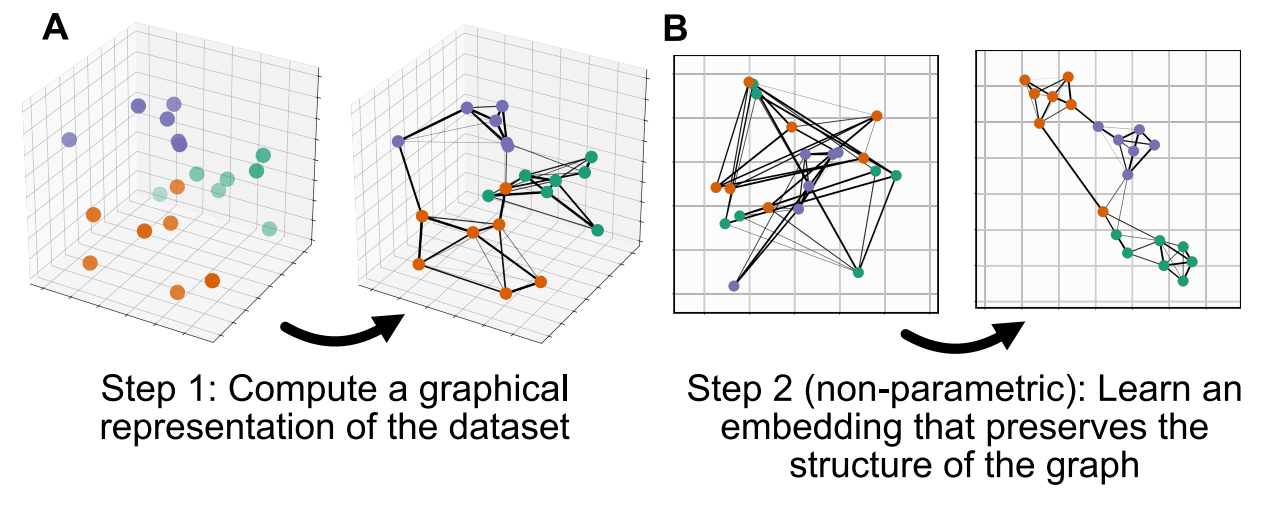
\includegraphics[width = \textwidth]{src/imgs/umap-explanation.png}
    \caption{Source: \cite{sainburg2021parametric}. UMAP dimensionality reduction process. The \textit{non-parametric} method is the method described in this work.}
    \label{fig:umap_explanation}
\end{figure}

\subsubsection{Uniform Manifold Approximation and Projection}
%
UMAP is a recent method from~\cite{mcinnes2020umap} that competes with t-SNE the status of state of art in dimensionality reduction.
%
The presentation of the method will be based on the introduction made in~\cite{coenen2018umap}.
%

The process of space transforming from UMAP can be divided into two steps as shown in Figure~\ref{fig:umap_explanation}: the creation of a graph with the high-dimensional data, and the representation of this graph in low-dimension. 
%
In the example, 3D data is transformed to be plotted in 2D.
%
The graph is formed from the data points as vertices, and the weighted edge between two vertices indicates the connectedness of the points.
%
To construct this graph, from each point a radius is drawn, 
%
other points inside this radius are considered connected to the initial point,
%
the length is this radius must be adequate to avoid isolated points and avoid connect all points.
%
For that reason, it is based on the distance between the point and its $n$-th nearest neighbor.
%
Points that are inside this radius and closer to the initial point will have edges with bigger weights than points that are also inside the radius, but farther from the center.
%
After this graph is built in high-space, an optimization process is used to generate a similar layout of points in a low-dimensional space.
%

The two parameters that affect the projection obtained from UMAP are the \textit{number of neighbors} and the \textit{minimum distance}.
%
As already mentioned above, the number of neighbors is used in constructing the graph in high-dimension, 
%
when the number of neighbors considered is high, more connections between points will be created, and the graph will represent more the global structure of the data,
%
when it is low, the method will give more importance to local patterns of the data, as only really close points will be connected.
%
The other parameter is used in the construction of the low-dimensional representation, it is the minimum distance between two points in the new space,
%
when its value is low, points will be close together,
%
when it is high, points will have more freedom to arrange themselves but can lead to noisy results.
%

UMAP presents really good results in different patterns of high-dimensional data.
%
However, due to having two parameters,
%
to obtain good results for a specific dataset is necessary to try different combinations of parameters and analyze the different results.
%

\subsection{Spatial indexing}

As defined by~\cite{azri2013review}, spatial indexing is a technique to optimize query processing in large spatial databases,
%
it organizes rows of information on memory in such a manner that search is efficient.
%
The use of spatial indexing methods for projection is because to make faster queries,
%
the structures built need to preserve proximity between points, 
%
creating a good representation of the space that can be traversed to get a 1D projection.
%
It can be divided into two categories, space driven structures, that are dependent only on the space of the data, 
%
and data-driven structures, that depending on the points used, will generate different structures.
%
Examples of space-driven structures are trees such as Quadtree and KD-Tree, and space-filling curves that will be presented in this work.
%

With the proof of George Cantor that the interval $[0, 1]$ can be mapped bijectively to the unit square $[0, 1] \times [0, 1]$ in 1878, 
%
the discussion if this map could be continuous started, with the following result by E. Netto that if the map is bijective, it is necessarily discontinuous. The remaining question was if there could be a surjective and continuous map.
%
In 1890 Giuseppe Peano answered this question by constructing a function that had this property~\cite{sagan2012space}.

%
Now called space-filling curves, they are functions $f : [0, 1] \to [0, 1]^2$ that for each $(x, y) \in [0, 1]^2$, there is $z \in [0, 1]$ such that $f(z) = (x, y)$.
%
They are generally defined by a limit of functions that are not surjective in the unit square, but when the limit is applied, it can be shown that is convergent and the resulting function is space-filling.

%
In this text, we will focus on the geometric interpretation of space-filling curves. They can be generated by a process that is recursive and self-similar, exemplified in Figures~\ref{fig:hilbert-curve} and \ref{fig:morton-curve}.
%
Although not being one of the objectives when were created, these curves present a property that close points in the interval will be mapped to neighborhoods in the unit square, a characteristic that is highly useful in computational sciences to build data structures (spatial indexing) or in algorithms \cite{bader2012space}.

\subsubsection{Hilbert curve}

Hilbert-curve is a space-filling curve proposed by David Hilbert in 1891 \cite{Hubert1891}. The curves of order from 1 to 6 can be seen in Fig.~\ref{fig:hilbert-curve}.
%
The iterative process of creating the Hilbert curve starts by dividing the unite square into four smaller squares, as shown in the curve of order 1,
%
then these squares are traversed by following a format of an upside-down \textit{U},
%
the green line represents the curve of order 1.
%
To get the curve of order 2, each of the four smaller squares from the previous curve is divided again into 4 equal parts.
%
In each of them, a curve of order 1 is placed, 
%
in the image there are two copies in color green exhibited,
%
the other two copies are not so easily identified because they are rotated to connect with the remaining of the line without self-crossing.
%
The curves of bigger order are created in the same manner: dividing each square in 4, and connecting 4 copies of the curve of the previous order, two in the same orientation and two rotated.
%
In the figure, there are indications of one of the copies for curves of orders 3 and 4.
%

To obtain a projection of data $Y \in \mathbb{R}^{m \times 2}$, the first step is to move the data to the unit-square, 
%
this can be done by just subtracting the minimum and dividing by the range in each of the two dimensions.
%
Now the curve is traversed, by determining a start point (on the figure, the bottom left),
%
and walking through the unit square, each of the smaller squares is numbered by the order of passing.
%
In the example of the curve of order 1, the square $[0, 0.25]^2$ receives the number 1 because of being the first visited,
%
the square $[0, 0.25] \times [0.25, 0.5]$ is the second visited and receives the number 2.
%
In the image, there are some examples of numbering for curves of orders 2 and 3.
%
For the data points, the projection value is the number of the square that is contained.
%

The projected data $Z$ will be discrete, i.e., $z_i \in \mathbb{Z}$, and with the order of the curve being $k$, the maximum value obtained will be $4^k$. 
%
Depending on the application, these projection values can be divided for $4^k$, obtaining that $z_i \in [0, 1]$.


\begin{figure}
    \centering
    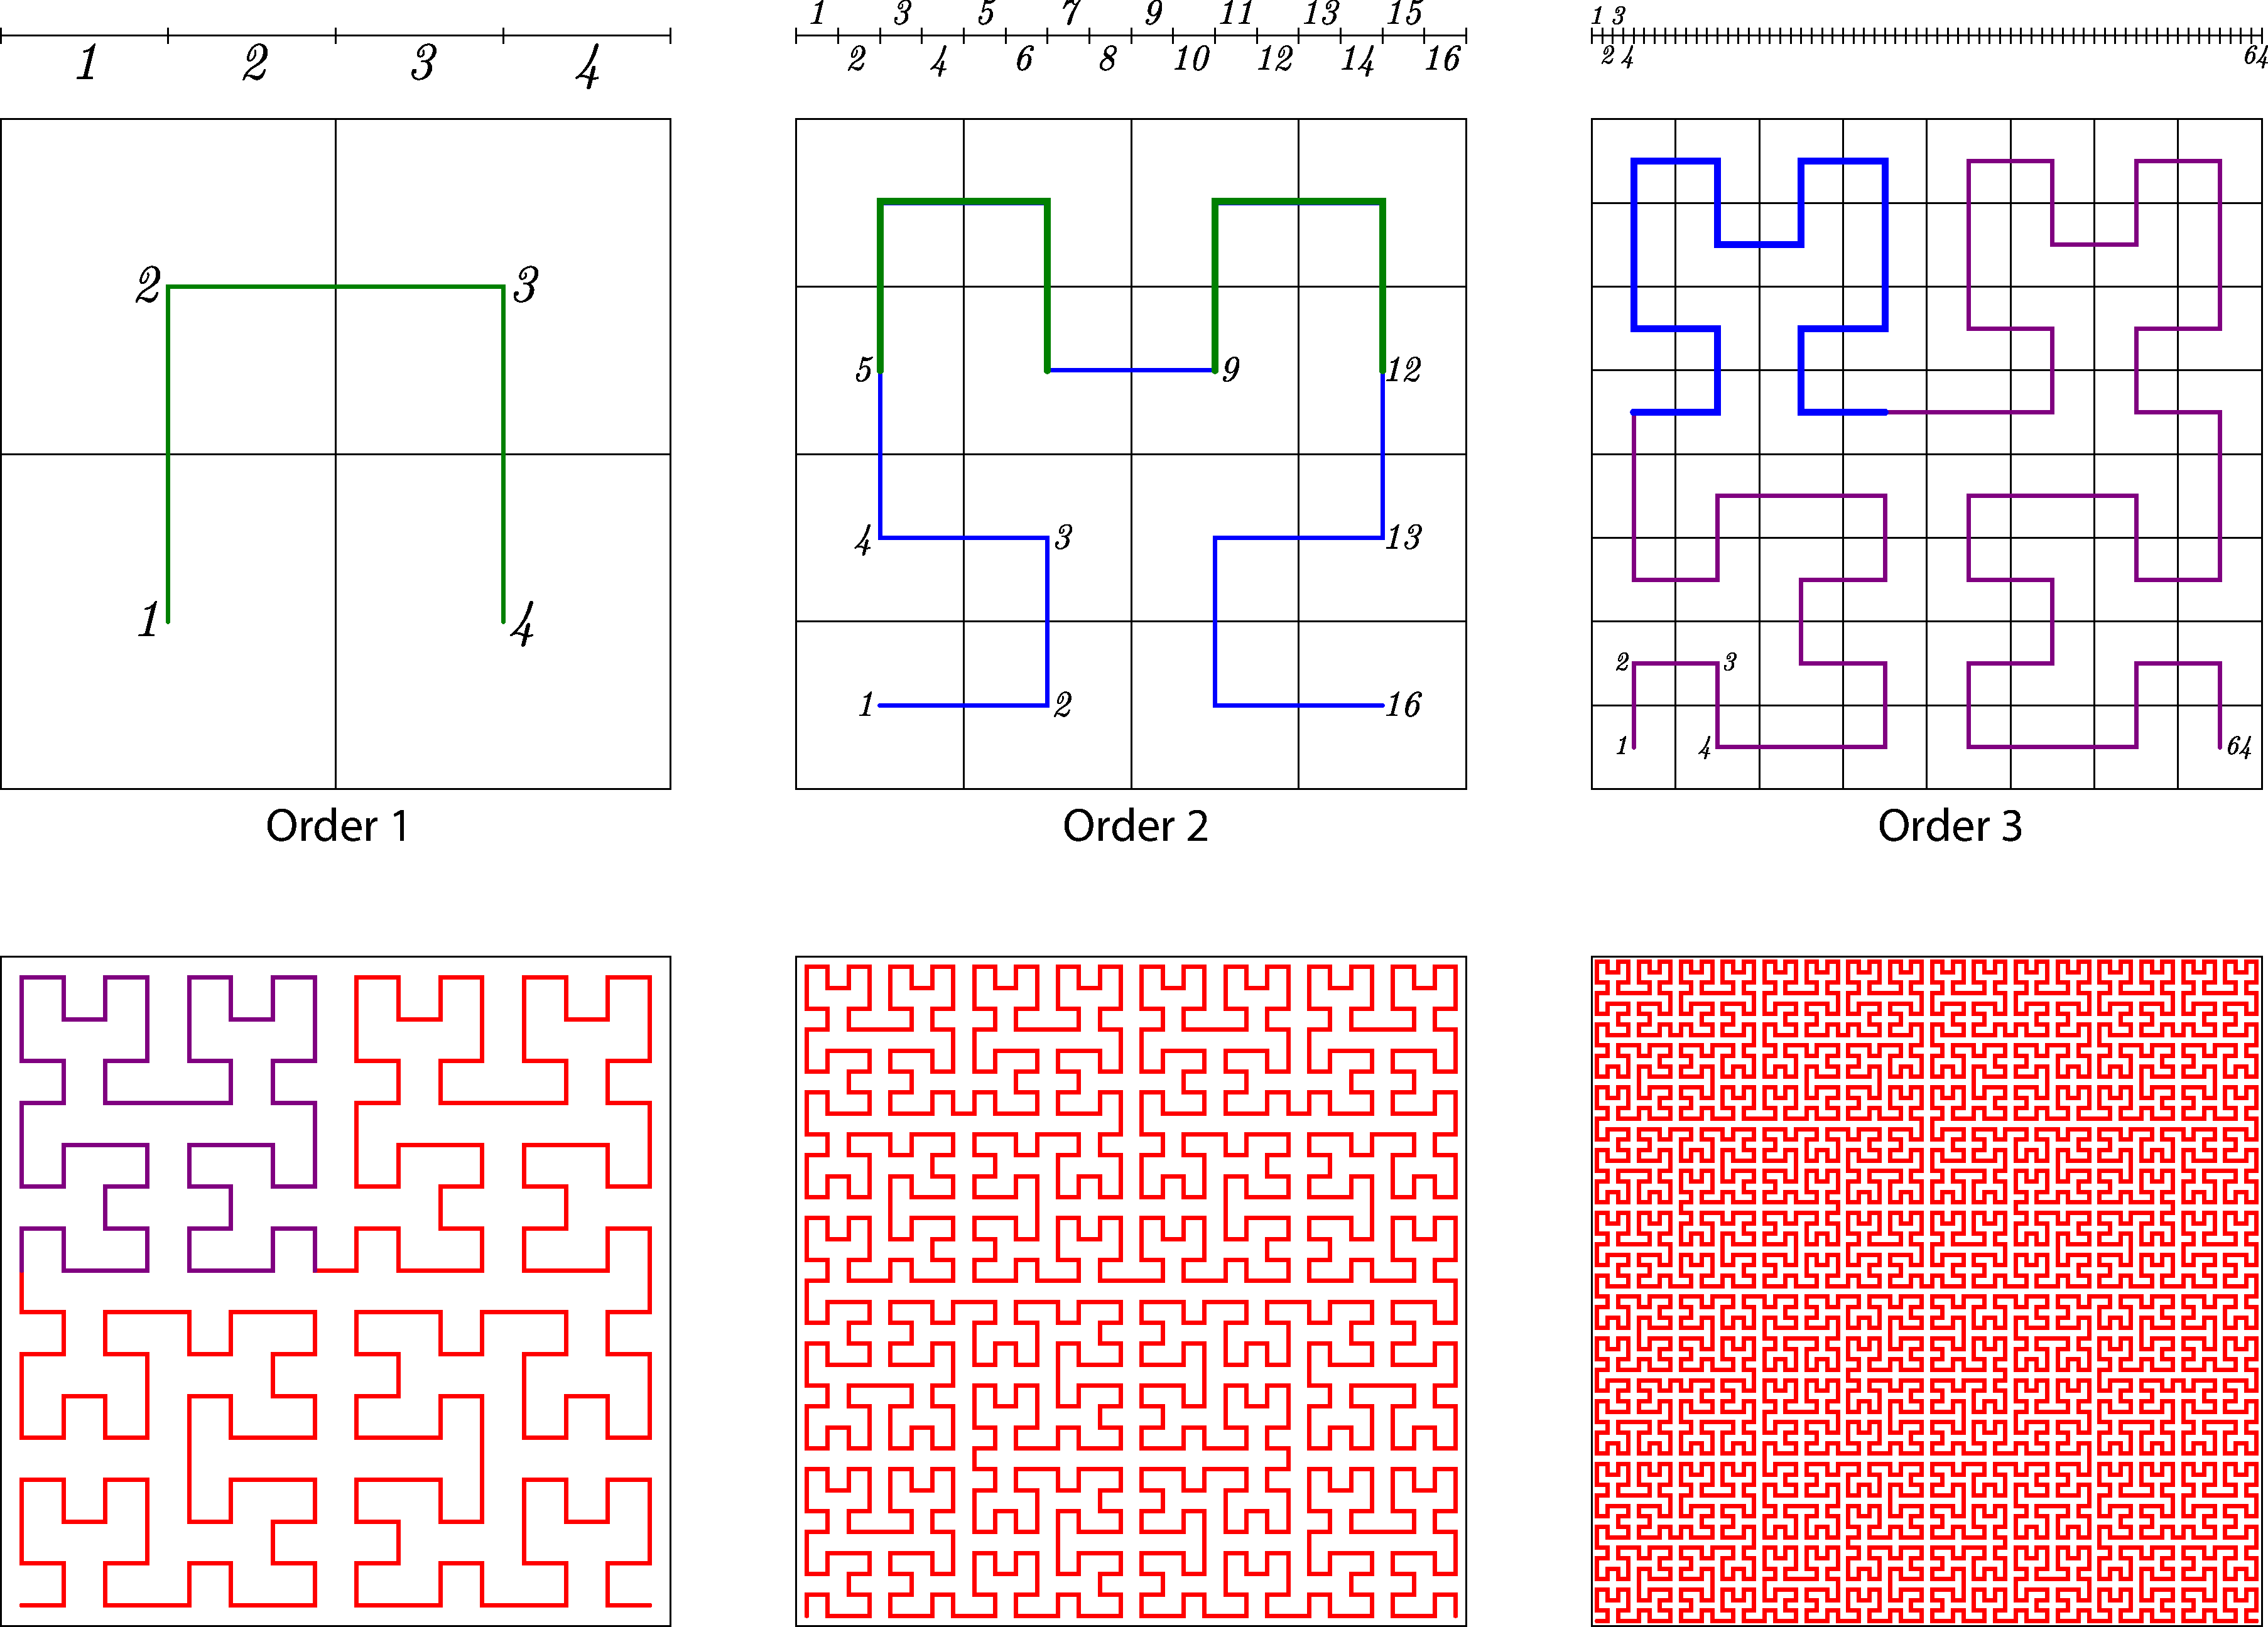
\includegraphics[width = \linewidth]{src/imgs/hilbert-curve.pdf}
    \caption{Source: Braindrain0000, CC BY-SA 3.0 \url{<http://creativecommons.org/licenses/by-sa/3.0/>}, via Wikimedia Commons, adapted by the author. Hilbert curves of a different order, the numbers beside the curves indicate the projected value represented by the square, and the change of colors in the same curve highlight the shape of the curve of the previous order.}
    \label{fig:hilbert-curve}
\end{figure}

\begin{figure}
    \centering
    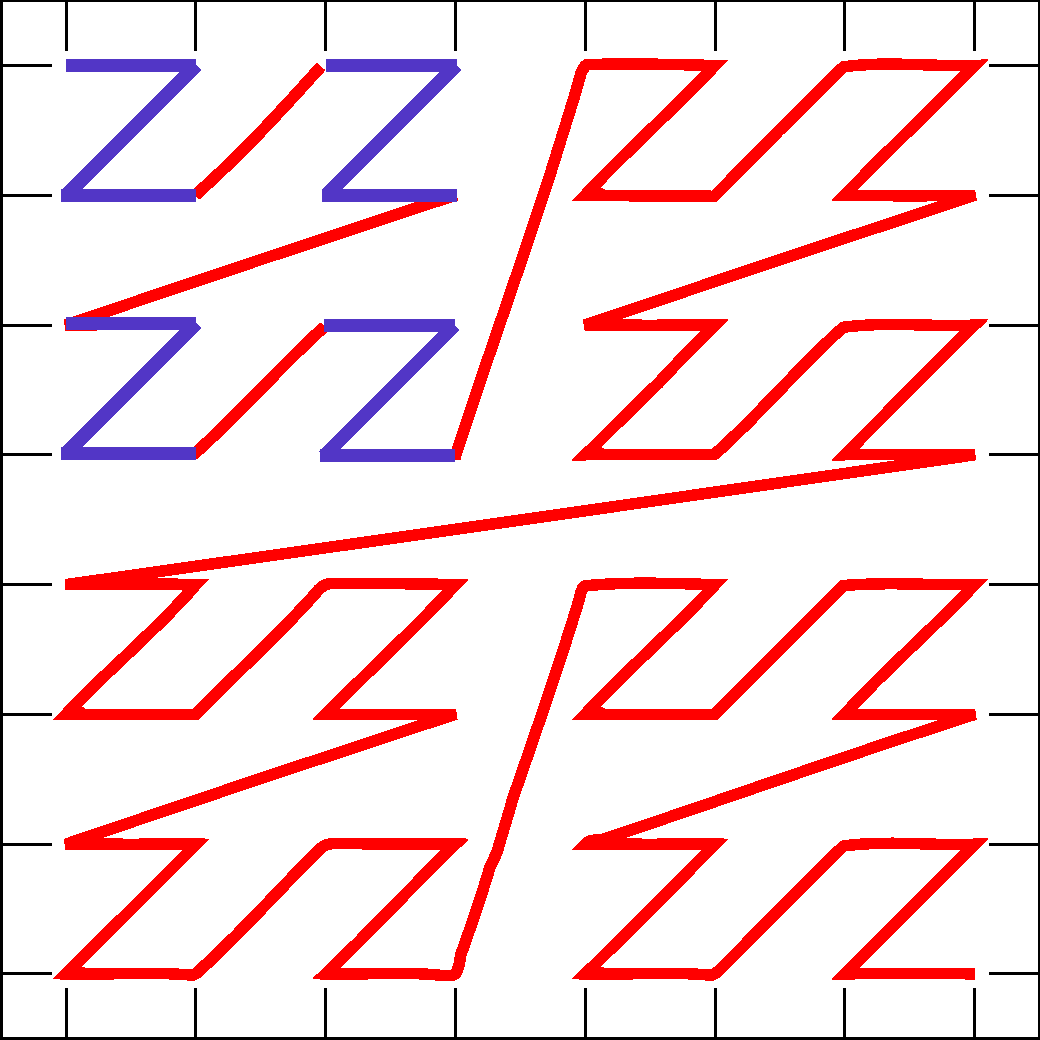
\includegraphics[width = 0.5\linewidth]{src/imgs/morton-curve.pdf}
    \caption{Source: Public domain, adapted by the author. Morton curve of order 3, on the top left corner, a curve of order 2 is built with 4 copies of the curve of order 1 that are colored with blue..}
    \label{fig:morton-curve}
\end{figure}

\subsubsection{Morton curve} 

The Morton curve, shown in Figure~\ref{fig:morton-curve}, is very similar to the Hilbert curve, with the same process of generation, by dividing in 4 and replicating previous curves.
%
Despite, the curve of order 1 does not have the upside-down \textit{U} shape, it has a \textit{Z} shape, and for that reason is commonly called of Z-Order curve.
%
Another difference is that the copies of the curve are not rotated.
%
In the Figure, the 4 copies of the curve of order 1 that are used to create the curve of order 2 are marked with blue color.

A projection can be made with the Morton curve with the same process described to project with the Hilbert curve.
%

Many other space-filling curves exist and are used for spatial-indexing, although,
%
the present work will only consider the Hilbert and Morton curve due to the big number of already considered projection methods 
%
and their prevalence in applications.

\section{Clustering}
\label{sec:clustering}

Clustering is a very common unsupervised method for data mining \cite{ansari2020spatiotemporal}, the objective is to separate data points in groups that are similar and, in some cases, noise points.
%
In the context of spatio-temporal data, there is the necessity of the adaptation of methods due to the different nature of distance in the spatial and temporal dimensions. 
%
While time is 1D, the space is 2D, and there is no simple relation between our measurements of time (seconds, hours, days) and our measurements of space (meter, kilometer, degree), so when searching for neighborhoods, these two subsets of the attributes of the data must be handled differently.
%
Adapted methods were already proposed and \cite{ansari2020spatiotemporal} present a review of them.
%
In this section, it is presented the method ST-DBSCAN, a variation of the method DBSCAN~\cite{ester1996density} for spatio-temporal data, and was used in this work to identify events.
%

\subsection{DBSCAN}
DBSCAN was proposed by \cite{ester1996density} and still today one of the most used methods, with many adaptations, improvements, and experimentation.
%
The idea is that a cluster of points presents a higher density inside than outside of it, and that this density is related to the number of neighbors of each point. Some definitions from the original article will now be presented:
%

\textbf{Neighborhood of a point} For a set of points $D$, a point $p$ and distance function $d$, the neighborhood of $p$ with threshold $Eps$ is $N_{Eps}(p) = \{ q | d(p, q) \leq Eps, q \in D \}$. The sub index of $N_{Eps}(p)$ will be omitted.
%

\textbf{Directly density-reachable} A point $p$ is directly density-reachable from $q$ if $p \in N(q)$ and $N(q) \geq MinPts$.
%

\textbf{Density-reachable} A point $p$ is density-reachable from a $q$ if there is a sequence of points $p, p_1, \dots, p_k, q$ such that consecutive points are directly density-reachable.
%

\textbf{Density-connected} Two points $r$ and $s$ are density-connected if there is a point $p$ such that both are density-reachable to $p$.
%

The intention of the previous definition was to construct the idea of a cluster.  
%
Points from the same neighborhood would be included in the same cluster, but it is a restrict constraint, so points that density-reachable will also be considered in the same cluster, and as it is difficult to happen between border points, points density-connected are also considered to be in the same cluster.
%

\textbf{Cluster} Let $D$ be a database of points, a cluster $C$ with thresholds $Eps$ and $MinPts$ is a non-empty subset of $D$ if:
\begin{itemize}
    \item $\forall p, q \in D$ if $p$ is density reachable from $q$ and and $p \in C \implies q \in C$.
    \item $\forall p, q \in C$, $p$ and $q$ are density-connected.
\end{itemize}
%

To compute clusters according to the previous definition, the algorithm iterates over points, calculating the neighborhood and verifying if the number of points is bigger than $MinPts$, then each point of the neighborhood is added to a stack, and for each point $q$ in the stack, the neighborhood is calculated and the size verified, if it is bigger than $MinPts$, all points are added to the stack, and this process repeats until the stack is emptied.

\subsection{ST-DBSCAN}

The now presented method ST-DBSCAN~\cite{BIRANT2007208} improves DBSCAN by initially considering two thresholds $Eps_1, Eps_2$ for the neighborhood, with $Eps_1$ being the threshold for the spatial variables and $Eps_2$ the threshold for time variables. Another adaptation is the addition of a parameter $\Delta \varepsilon$ that limits the search for density-reachable points, the distance between the mean of non-spatial attributes of points from a cluster $C$ and a new point $q$ should be smaller than $\Delta \varepsilon$ to be considered the same cluster. The algorithm is present in \ref{alg:dbscan}.

\begin{algorithm}[H]
\label{alg:dbscan}
\SetAlgoLined
\SetKwInOut{Input}{Input}
\Input{
$D$ - set of objects \\
$Eps_1$ - threshold for spatial distance in neighborhood \\
$Eps_2$ - threshold for temporal distance in neighborhood \\
$MinPts$ - threshold for the number of points to consider a cluster \\
$\Delta \varepsilon$ - threshold to verify when adding to cluster 
}
\SetKwInOut{Output}{Output}
\Output{
$C$ - array with cluster id for each point, value $-1$ for noise points
}
cluster\_label $= 0$ \;
\For{$p \in D$}{
\If{$p$ not in a cluster}{
$N = $ retrieve\_neighbors$(p, Eps_1, Eps_2)$\;
\uIf{$|N| < MinPts$}{
Mark $p$ as noise \;
}
\uElse{
cluster\_label++\;
\For{$q \in N$}{
Mark $q$ as cluster\_label\;
}
stack $= N$\;
\While{stack is not empty}{
q = stack.pop()\;
$N_q =$ retrieve\_neighbors$(q, Eps_1, Eps_2)$\;
\If{$|N_q| >= MinPts$}{
\For{$s \in N_q$}{
\If{($s$ not in a cluster) 
and (distance\_cluster\_center$(s) \leq \Delta \varepsilon$) }{
Mark $s$ as cluster\_label\;
stack.add($s$)\;
}
}
}
}
}
}
}
\caption{ST-DBSCAN}
\end{algorithm}

